%% Copyright 2006-2015 Xavier Danaux (xdanaux@gmail.com).
%
% This work may be distributed and/or modified under the
% conditions of the LaTeX Project Public License version 1.3c,
% available at http://www.latex-project.org/lppl/.


\documentclass[11pt,letterpaper,sans,dvipsnames]{moderncv}        % possible options include font size ('10pt', '11pt' and '12pt'), paper size ('a4paper', 'letterpaper', 'a5paper', 'legalpaper', 'executivepaper' and 'landscape') and font family ('sans' and 'roman')

\usepackage{fancyhdr}
\usepackage{xcolor}
\chead{\color{RoyalBlue}G. T. Antell, PhD}
% \cfoot{Page \thepage\ of \pageref{LastPage}}

% moderncv themes
\moderncvstyle{fancy}                             % style options are 'casual' (default), 'classic', 'banking', 'oldstyle' and 'fancy'
\moderncvcolor{blue}                               % color options 'black', 'blue' (default), 'burgundy', 'green', 'grey', 'orange', 'purple' and 'red'
%\renewcommand{\familydefault}{\sfdefault}         % to set the default font; use '\sfdefault' for the default sans serif font, '\rmdefault' for the default roman one, or any tex font name

% \nopagenumbers{}                                  % uncomment to suppress automatic page numbering for CVs longer than one page

% character encoding
\usepackage[utf8]{inputenc}                       % if you are not using xelatex ou lualatex, replace by the encoding you are using

% adjust the page margins
\usepackage[scale=0.78,top=1in,bottom=1in]{geometry}
%\setlength{\hintscolumnwidth}{3cm}                % if you want to change the width of the column with the dates
%\setlength{\makecvtitlenamewidth}{10cm}           % for the 'classic' style, if you want to force the width allocated to your name and avoid line breaks. be careful though, the length is normally calculated to avoid any overlap with your personal info; use this at your own typographical risks...

\hyphenpenalty=10000

% personal data
\name{Gawain T.}{Antell, PhD}
% \title{Resumé title}             
%\address{Geology 1242 \\ 900 University Ave.}{Riverside, CA 92521}{}% "postcode city" and "country" arguments can be omitted or provided empty
\email{gawain.antell\\@ucr.edu}                           
% \phone[mobile]{}      % the optional "type" of the phone can be "mobile" (default), "fixed" or "fax"
%\homepage{gawainantell.com}                    
%\social[linkedin]{john.doe}                 
% \social[twitter]{GawainAntell}        
%\social[github]{GawainAntell}        
% \extrainfo{additional information}    
% \photo[64pt][0.4pt]{Antell_profile_small}              % '64pt' is the height the picture must be resized to, 0.4pt is the thickness of the frame around it (put it to 0pt for no frame) and 'picture' is the name of the picture file
% \quote{Some quote}     

\usepackage[backend=biber, isbn=false, bibstyle=numeric, sorting=none, defernumbers=true, maxbibnames=50]{biblatex} 
\bibliography{presentations_publications.bib}

  
% bibliography with mutiple entries
%\usepackage{multibib}
%\newcites{book,misc}{{Books},{Others}}

%----------------------------------------------------------------------------------
%            content
%----------------------------------------------------------------------------------
\begin{document}

\thispagestyle{empty}

\makecvtitle

\section{Education}
\cventry{2017--2021}{DPhil}{University of Oxford}{UK}{}{Departments of Earth Sciences and Zoology. Defended Jan 2022 with no corrections.}  % arguments 3 to 6 can be left empty
\cventry{2012--2016}{B.S.}{Yale University}{USA}{\textit{magna cum laude}}{Ecology \& Evolutionary Biology (with distinction) and Geology \& Geophysics}

\section{PhD thesis}
\cvitem{Title}{\emph{Macroecological consequences of biotic and abiotic factors in marine communities through time}}
\cvitem{Supervisors}{Erin Saupe (Earth Sciences) \& Tim Coulson (Zoology)}
\cvitem{Research interests}{ % 
\begin{itemize}
\item Biodiversity across spatial, temporal, and taxonomic scales
\item Macroecology, marine biology, and invertebrate paleontology
\item Inferential statistics on time series and spatial data
\end{itemize}
}

\section{Employment}
\cventry{from 2024}{Assistant Professor of Physical Geography}{Geography}{UCLA}{}{}

\cventry{2022--Present}{UC President's Postdoctoral Fellowship Program (PPFP)}{Earth \& Planetary Sciences}{University of California, Riverside}{}{Independent research fellowship; mentorship as part of the diversifying faculty initiative.}

\cventry{2022}{Postdoctoral Research Assistant}{Earth Sciences}{Oxford}{}{Grant-funded by UK Natural Environment Research Council to develop analysis software.}

\cventry{2016--2017}{Geoscientists-in-the-Parks Intern}{US National Park Service, Geologic Resources Division}{Florissant National Monument}{CO}{}
% Published independent research, assisted exhibit design, and surveyed geoheritage resources.

\cventry{2013--2016}{Collections Assistant}{Yale Peabody Museum of Natural History, Invertebrate Paleontology Division}{New Haven}{CT}{}
% Described new fossil species, cataloged specimens, and hosted public tours.

% \section{Leadership}
% \pagebreak

% bibliography
\nocite{*}
\printbibliography[type=article, title={Publications}] % , resetnumbers=true

\section{Other writing}
% \printbibliography[type=misc, title={Other writing}, resetnumbers=true]
\cvitem{}{(Not peer-reviewed.)}
\cvitem{}{\textbf{G Antell}. ``Why I changed my name, according to Latin taxonomy.'' Transpositions blog, \textit{International Society of Nonbinary Scientists} (2023). \href{https://isnbs.org/2023/08/18/why-i-changed-my-name-according-to-the-rules-of-latin-taxonomy}{isnbs.org/2023/08}.}
\cvitem{}{S Greene, \textbf{G Antell}, \textit{et al.} ``Safety and belonging in the field: a checklist for educators.'' \textit{EarthArXiv (2021).} \href{https://doi.org/10.31223/X53P6H}{DOI: 10.31223/X53P6H}.}
\cvitem{}{\textbf{G Antell}. ``All colours of pride.'' Rainbow Research blog series, journal of \textit{Methods in Ecology \& Evolution} (2021). \href{https://methodsblog.com/2021/06/28/rainbow-research-all-colours-of-pride/}{URL: methodsblog.com/2021/06/28}.}
\cvitem{}{B Fernando and \textbf{G Antell}. ``Recommendations for improving racial equality, diversity, and inclusion in the Department of Earth Sciences, University of Oxford.'' Public report (2021). Available at: \href{https://www.earth.ox.ac.uk/2020/06/department-of-earth-sciences-releases-report-of-ad-hoc-working-group-on-bame-issues/}{\textit{https://www.earth.ox.ac.uk/2020/06}}.}

\section{Invited talks}
\cvitemwithcomment{Stanford}{Dept.\ of Geological Sciences}{Apr 2023}
\cvitemwithcomment{UC Riverside}{Environmental Dynamics and GeoEcology Institute}{Mar 2023}
\cvitemwithcomment{U.\ of Southern California}{Paleo/Environmental seminar series}{Jan 2023}
\cvitemwithcomment{UC Riverside}{Dept.\ of Earth \& Planetary Sciences}{Jan 2023}
\cvitemwithcomment{UC Los Angeles}{Dept.\ of Earth, Planetary \& Space Science}{Sep 2022}
\cvitemwithcomment{Sheffield University}{Ecology \& Conservation series}{Oct 2021}
\cvitemwithcomment{Yale}{Earth and Planetary Sciences}{May 2021}
\cvitemwithcomment{Harvard}{MCZ and Dept.\ Organismic \& Evo.\ Bio.\ paleobiology labs}{Nov 2020}
\cvitem{EDI talk}{``Decolonizing ecology and conservation science,'' Zoological Society of London (Feb 2021) and Oxford Zoology Dept.\ (July 2020).}
\cvitemwithcomment{Oxford Museum of Natural History}{Public research lecture}{Jan 2020}
\cvitemwithcomment{Oxford Geology Group}{Student speaker at annual symposium}{Mar 2019}
% \cvitem{Alumni speaker}{Yale Peabody Museum 150th Anniversary Symposium. One of two recent undergraduate speakers, Verrill Medal symposium, 2016.}

\pagebreak

\section{Awards}
\subsection{Scholarships}
\cvitemwithcomment{}{President's Postdoctoral Fellowship, U.\ of California}{2022--2024}
\cvitemwithcomment{}{Clarendon Fund Scholarship}{2017--2021}
\cvitemwithcomment{}{St John's College Alumni Scholarship}{2017--2021}
\cvitemwithcomment{}{NSF Graduate Research Fellowship Program (declined)}{2017}
\cvitemwithcomment{}{Jerry (1953) and Jackie Inskeep Scholarship Fund}{2013--2016}
\cvitemwithcomment{}{Summer Environmental Fellowship, Yale}{2014}
\cvitemwithcomment{}{US National Merit Scholarship}{2012}
\subsection{Grants}
\cvitemwithcomment{}{Burdett-Coutts Grant, Earth Sciences, of Oxford (\pounds 1,650)}{2019}
\cvitemwithcomment{}{Postgraduate Special Grant, St John's College (\pounds 1,250)}{2018}
\cvitemwithcomment{}{Travel Grant, Palaeontological Association (\pounds 300)}{2018}
\cvitem{}{Ernst Mayr travel grant for animal systematics, Museum of Comparative Zoology, Harvard University (\$1,100) \hspace{18 pc} {\small \textit{2016}}}
% \cvitemwithcomment{}{Pierson College Richter Fellowship (\$500)}{2015}
\cvitemwithcomment{}{Yale Science Center Int'l Fellowship (\$3,870; \$4,300)}{2014, 2015}
\cvitemwithcomment{}{Yale Freshmen Summer STEM Research Fellowship (\$4,300)}{2013}
\subsection{Awards}
\cvitem{}{Winifred Goldring Award for outstanding paleontology PhD student; conferred by Association for Women Geoscientists and Paleontological Society \hspace{4 pc} {\small \textit{2021}}}
\cvitemwithcomment{}{1st-place student talk in Geobiology \& Geomicrobiology, GSA meeting}{2020}
\cvitemwithcomment{}{Oxford Earth Sciences award for equality, diversity, \& inclusion}{2020}
\cvitemwithcomment{}{1st-place student talk, North American Paleontological Convention}{2019}
\cvitem{}{D.\ E.\ Chantler Award for ``the Yale Senior who has best exemplified qualities of courage, strength of character, and high moral purpose'' \hspace{7 pc} {\small \textit{2016}}} % Yale 
\cvitemwithcomment{}{W. R. Belknap Prize for excellence in a biology thesis, Yale}{2016}
\cvitemwithcomment{}{1st-place student speed talk, Connecticut Entomological Society}{2015}
% commended talk, CPEG

\section{Software}
\cvitem{divvy}{Developed an R package to spatially subsample biodiversity data, for fair comparisons through time and across environments (Antell \textit{et al.} 2020, 2024).}
\cvitem{kerneval}{Developed an R package for kernel density estimation that corrects density curves for biased observation/sampling (Antell \textit{et al.} 2021).}
\cvitem{Install at}{\href{https://cran.r-project.org/package=divvy}{cran.r-project.org/package=divvy}; \href{https://github.com/GawainAntell/kerneval}{github.com/GawainAntell/kerneval}}
\hfill 
{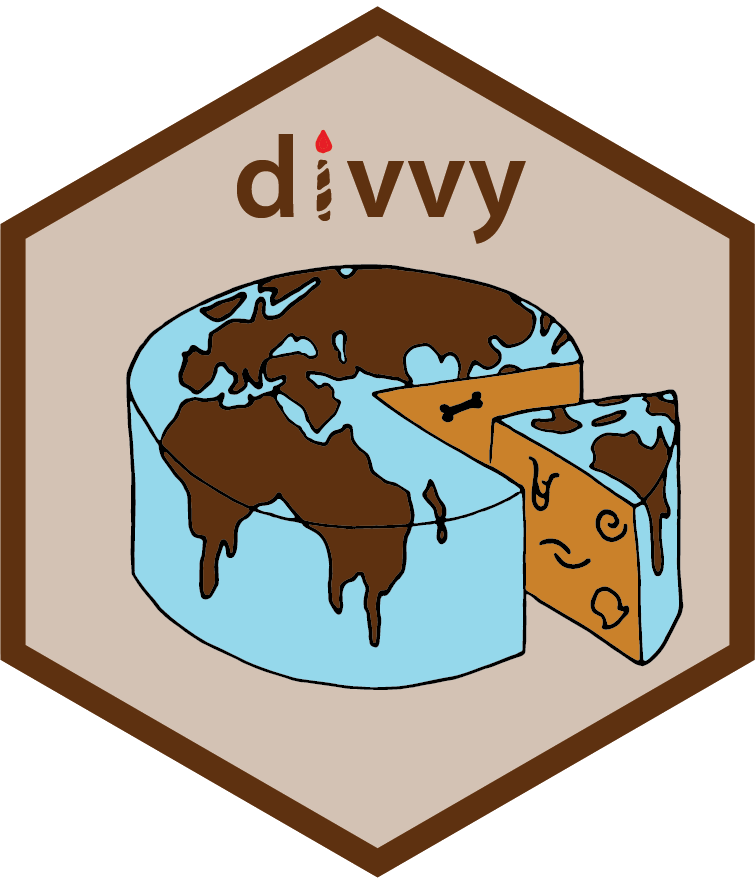
\includegraphics[width=2.3cm]{divvy_logo}}
{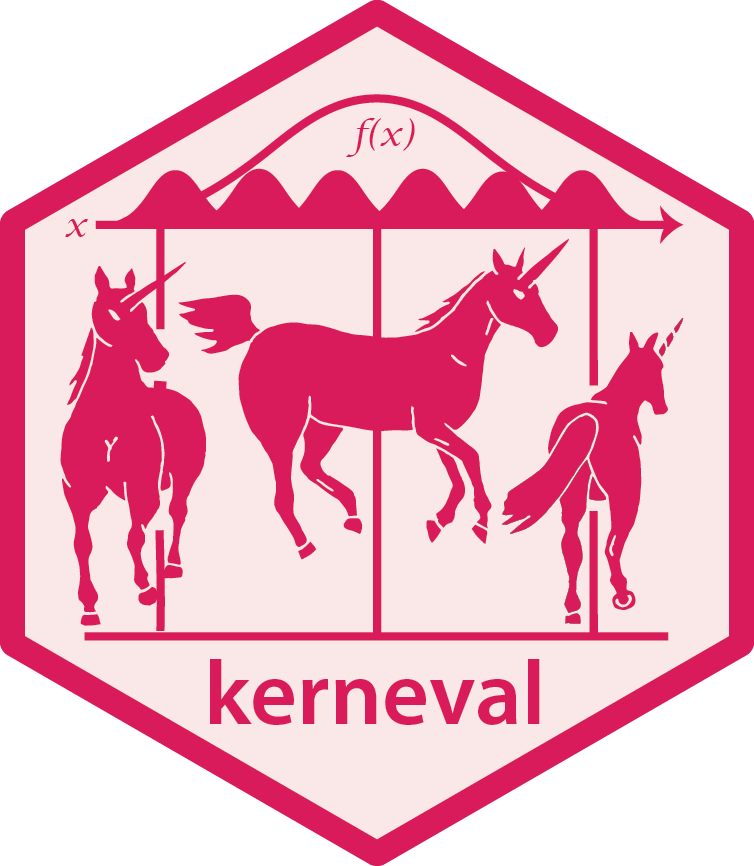
\includegraphics[width=2.3cm]{kerneval_logo}}

\pagebreak

% Conference talks
\printbibliography[type=inproceedings, title={Conference talks}, resetnumbers=true] 

\section{Certifications \& training}
\cvitem{Faculty Success Program}{National Center for Faculty Diversity \& Development 12-week "bootcamp" program for minoritized faculty. Remote, 2023.}
\cvitem{Teaching certification}{SEDA Supporting Learning award in higher education (Descriptor 1 of  UK Professional Standards Framework), 2020.}
\cvitem{Science communication and science policy}{``Reclaiming STEM'' 4-part workshop series, run by and for minorities in STEM. Held remotely, 2020.}
\cvitem{Wilderness First Responder}{80-hour emergency medicine certification with wilderness upgrade, maintained valid 2017--Present.}
\cvitem{Science communication for children; STEM Ambassador training; University teaching}{Individual workshops, University of Oxford, Jan--Feb 2019.}
\cvitem{Stratigraphic paleobiology}{Paleo.\ Society 2-wk grad field course. MT, 2017.} % Bitterroot Mountains. Sequence strat.\ and logging sections.

\section{Teaching}
\cvitem{Undergraduate lecture course}{guest lecturer for unit on climate change, 300 students, University of California, Riverside \hspace{13 pc}{\small \textit{2023}}}
% \cvitemwithcomment{Discussion seminar}{guest taught papers discussion on extinction}{2021}
\cvitemwithcomment{1st-yr Invertebrate Paleontology}{laboratory teaching assistant}{2017--2020}
\cvitemwithcomment{2nd-yr Invertebrate Paleontology}{laboratory teaching assistant}{2019, 2021}
\cvitemwithcomment{2nd-yr Past Environments}{laboratory teaching assistant}{2018, 2020}
\cvitemwithcomment{3rd-yr Quantitative Paleontology}{developed data analysis exercise}{2019}
\cvitem{Tutorials (small-class discussions)}{developed and led 4-part paleontology unit for 1st-yr students, St Peter's College. Assigned and assessed work. \hspace{3 pc}{\small \textit{2019}}}
\cvitem{Field instructor}{Earth Sciences undergraduate field course. Isle of Arran, UK. 1 week, 2019 (2020 cancelled due to COVID-19). Graded student maps.}
\cvitem{Field instructor}{Earth Sciences undergraduate course. Dorset, UK. 1 week, 2018, 2019, 2020 (virtual). Intro to sedimentary field skills; graded field notebooks.}
\cvitem{Field instructor}{Day course to local outcrops in South East England. 2019, 2022}

\section{Service}
\cvitem{Peer reviewer}{\textit{Global Ecology \& Biogeography, Science Advances, Paleobiology, Palaeontology, Am.\ Naturalist, Am.\ J.\ Botany, Royal Society and Nature families}}
\cvitem{Session chair}{Ocean Sciences Meeting, 2024, co-convener; Geological Society of America, 2022; Palaeontological Association, 2020.}
\cvitem{Membership}{Paleontological Society, Geological Society of America, International Association for Diversity in Geoscience, International Society of Nonbinary Scientists}
\cvitem{Student adjudicator}{Ocean Sciences Meeting, 2024. Geological Society of America meeting, 2022; reformed the scoring rubric for equity.}
\cvitem{Divisional EDI Fellow}{Inaugural fellow for Earth Sciences. Co-wrote strategic plan for EDI in Oxford division of Maths, Physical, \& Life Sciences, 2020-2021.}
\cvitem{Working group}{Co-chair for racial diversity and inclusion in Earth Sciences, Oxford, 2019--2020. Co-authored report of 42 action item recommendations.}
\cvitem{Graduate student representative}{Divisional committee for Graduates, 2018--2020. Dept.\ committees for Equality, Graduate Students, and Teaching, 2017--2021. Graduate President serving 9 committees of St John's College, 2017--2018.}

\end{document}


%% end of file `template.tex'.
